\chapter{Distribution}
\label{ch:distrib}


\section{Recherches}
Lors de cette partie du travail, une étude comparative a été effectuée pour essayer de trouver la base de distribution la plus adaptée aux besoins des utilisateurs de l'\textit{HEIG-VD}.
Tout d'abord, il a fallu évincer certaines distributions qui sont trop spécifiques, comme \textit{Kali Linux}, \textit{Parrot OS}.
En effet, certaines de ces distributions sont spécifiques au domaine de la sécurité et sont livrées avec beaucoup plus d'outils que nécessaire au bon fonctionnement d'un étudiant.
Il a alors été décidé de comparer les distributions principales :
\begin{itemize}
    \item Ubuntu
    \item Debian
    \item Manjaro
    \item Archlinux
\end{itemize}   
Le détail de cette comparaison se trouve ci-dessous :

\begin{figure}[H]
	\centering
	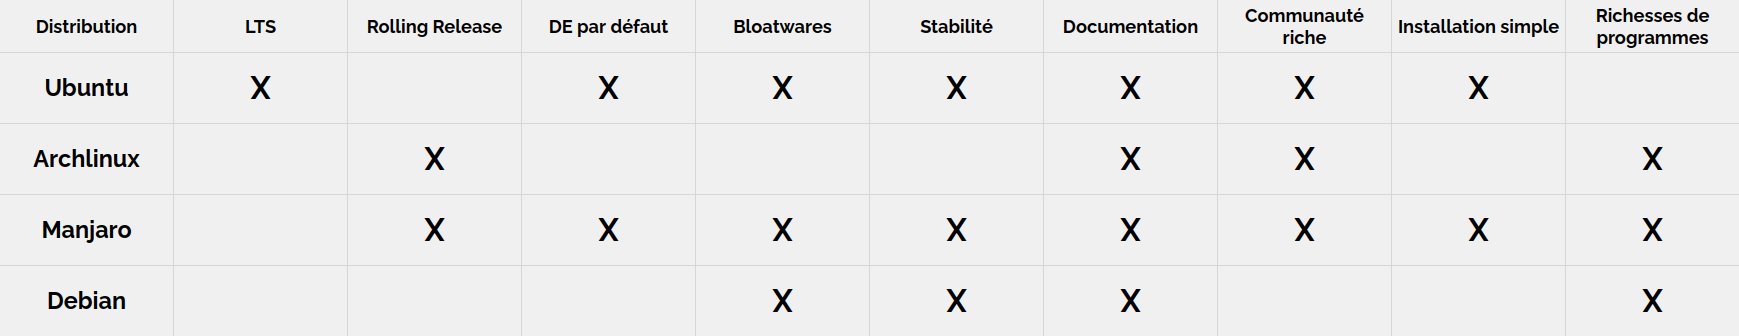
\includegraphics[scale=0.25]{images/distros_comp.png}
	\caption{Comparaisons des distributions}
	\label{fig:distros_comp}
\end{figure}


Le système de points est défini selon les critères suivants :
\begin{enumerate}
    \item Utilité
    \item Modularité
    \item Personnalisation
    \item Légèreté
\end{enumerate}

Finalement, Ubuntu est sorti comme choix de base de distribution. 
Le fait que cette distribution utilise un système de \acrfull{lts} permet de garantir une stabilité dans la compatibilité avec une multitude d'ordinateurs différents et ce de manière durable.
Les soucis principaux de cette distribution sont la surcouche \textit{\GLS{GNOME}} gérant le \acrfull{gui} et les logiciels installés de base.
Pour le dernier de ces problèmes, il a fallu trouver un moyen d'enlever un maximum de logiciels et librairies sans casser le système.
Au terme de certaines recherches, il a été déterminé que ces logiciels peuvent être ciblés et supprimés de manière aisée.
\newline
Concernant le soucis principal, l'utilisation de \GLS{GNOME}, il a fallu refaire une analyse comparative entre les \acrfull{de} principaux :
\begin{figure}[H]
	\centering
	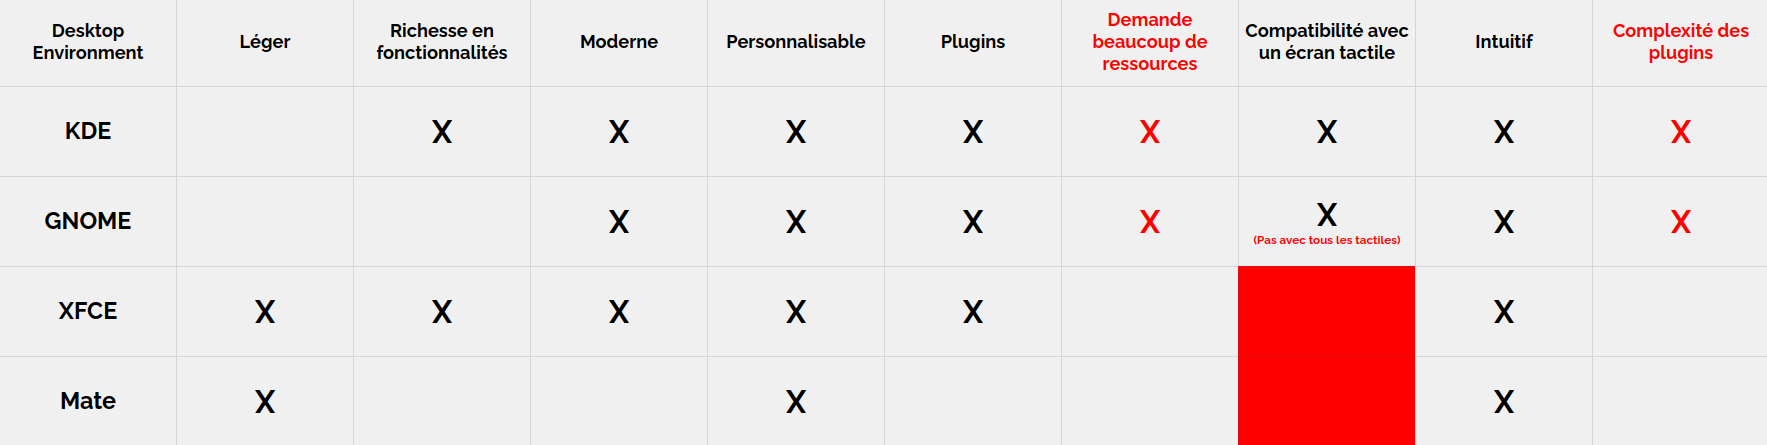
\includegraphics[scale=0.25]{images/DE_comp.png}
	\caption{Comparaisons des \acrfull{de}}
	\label{fig:de_comp}
\end{figure}
Il est possible de voir que seuls les principaux et les plus utilisés ont été mis en avant :	
\begin{itemize}
    \item KDE
    \item GNOME
    \item XFCE
    \item Mate
\end{itemize}
En effet, ces quatre \acrshort{de} font partie des plus utilisés et plus pratique pour un utilisateur lambda.
Il est en effet impératif de proposer une solution avec un \acrshort{gui} utilisable par n'importe quel utilisateur, c'est pourquoi des \acrshort{de} comme \textit{i3}, \textit{bspwm}, etc. ont été mis de côté.
Le système de points a été mis en place de manière à pouvoir classer de manière simple et efficace :
\begin{enumerate}
    \item Légèreté
    \item Efficacité
    \item Modularité
\end{enumerate}
Ces critères paraissent essentiels et peuvent englober plusieurs aspects différents, le tout permettant d'avoir un aperçu complet d'un \acrshort{de}.
Pour finir, il a été retenu que la surcouche \gls{GNOME} sera complètement supprimée de la base de distribution \textit{Ubuntu} et sera remplacée par \textit{XFCE}. 
\newline
Jusqu'à lors, il était relativement complexe de configurer les différents services de l'HEIG comme la connexion au réseau, le VPN, les imprimantes ou l'accès à \textit{eistore}.
L'idée serait de fournir une centralisation des identifiants HEIG afin de permettre la connexion aux services énoncés.
Grâce à une demande automatique du mot de passe lors du login, il sera alors possible de déverrouiller tous ces services et donc d'y accéder.
Un ajout potentiel pourrait être un script permettant de recevoir les notes présentes sur GAPS par message sur l'application Telegram.
Un aspect légal de cette proposition reste encore à voir.
L'API de Telegram permet de mettre en place un bot qui accepte les messages envoyés depuis un Terminal.
Sur ce bot, il est possible de récupérer certaines informations comme les notes d'une année en particulier, d'une matière en particulier ou même de mettre en place une tâche récurrente permettant d'avoir les différentiels à intervalle précis.


\section{Spécifications}

\subsection{Installateur}
Afin de pouvoir installer la distribution aux étudiants de l'HEIG-VD, un fichier \textit{.iso} sera fourni avec toutes les spécificités d'un installateur classique.
La distribution fournie sera configurée avec \textit{XFCE} et les logiciels superficiels seront désinstallés. 
\newline
Ensuite, afin de mettre le système courant sous forme ISO, \cite{ISO} il est possible de faire cela grâce à certaines commandes natives d'Ubuntu.

% TODO : Finir ça !!

\subsection{Scripts de centralisation}

Lors du premier démarrage après installation, un script Python fait une demande de saisie des identifiants AAI.
En effet, il est possible depuis Python de configurer des connexions aux réseaux grâce à \textit{nmcli}\cite{nmcli}.
Une connexion VPN peut être mise à disposition en utilisant l'écriture dans le fichier de configuration zsh, bash ou n'importe quel shell, créant ainsi un alias avec la bonne ligne de configuration.
L'utilisation de \textit{openconnect} comme VPN permet de simplifier l'accès au service.
La configuration de l'accès aux partages \textit{eistore} se fait de la même manière, un alias dans le fichier de configuration du shell.
Pour finir, les imprimantes peuvent être configurées grâce à l'outil \textit{lpadmin}. 
\newline
Le fait de faire une configuration comme cela permet d'éviter au maximum le stockage d'identifiants et de mots de passes.
Dans le cas des imprimantes et réseau sans fil, il n'y a pas d'autres alternatives que de configurer en dur dans le \gls{filesystem} la paire identifiants/mot de passe.
La localisation du stockage de ces derniers implique que seule une personne avec le mot de passe de la session et le mot de passe \textit{root} pourrait lire les informations.
Dans le cas des espaces \textit{eistore} et du VPN, le mot de passe sera demandé automatiquement lors de l'appel à ces alias et ne sera pas stocké sur l'ordinateur. 

\begin{figure}[H]
	\centering
	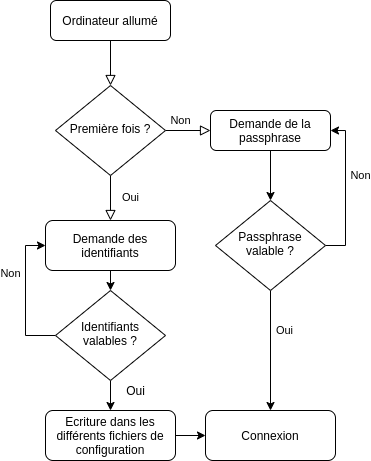
\includegraphics[scale=0.5]{images/centralisation.png}
	\caption{Demande des identifiants}
	\label{fig:central}
\end{figure}

\subsection{Notes et bot Telegram}
Pour cette partie, une configuration du bot existant \cite{bot} peut être configuré mais cela devra être fait manuellement.
Il est possible de fournir une automatisation du procédé de configuration mais elle ne parait pas optimisée ni sécurisée.
Pour se faire, il faut suivre la documentation fournie sur le dépôt mais qui va devoir être étoffée et complétée lors de ce travail.
Le bot est codé en Python et interagi avec Telegram grâce à l'API Telegram.
De plus, une discussion doit être engagée avec l'équipe s'occupant de Gaps, afin de pouvoir déterminer la légalité dans laquelle s'inscrit ledit script.

\section{Implémentation}

\subsection{Script de centralisation}
Ce script a pour but de configurer et faciliter l'accès aux différents services réseaux de l'HEIG-VD.
En effet, les imprimantes, les réseaux \textit{HEIG-VD} et \textit{eduroam}, le VPN et les dossiers partagés \textit{eistore}.
Le script complet se trouve en annexe et nous allons maintenant l'analyser.

\subsubsection{VPN}

\begin{listingsbox}{Python}{VPN}
file_path = expanduser("~/.zshrc")
file_object = open(file_path, 'a')
alias = "alias vpnHEIG=\"sudo openconnect --authgroup=All_Users --user=" +
username + " https://remote.heig-vd.ch\" \n"
file_object.write(alias)
\end{listingsbox}

Le script étant mis en place pour la distribution fournie lors de ce travail, il est assumé que l'utilisateur de ce script possède un terminal \textit{zsh}.
Cette partie du script écrit dans la configuration du terminal un alias qui permettra à l'utilisateur de lancer une connexion VPN vers le réseau de l'école.

\subsubsection{Réseaux}

Cette partie se décompose en deux fonctions :
\begin{itemize}
	\item la recherche de réseau
	\item la connexion au réseau
\end{itemize}

En effet, avant de pouvoir se connecter à un réseau, il faut vérifier qu'une connexion à ce réseau n'existe pas et si une interface réseau supportant le wifi soit disponible.

\begin{listingsbox}{Python}{Recherche de réseau}

\end{listingsbox}


\begin{listingsbox}{Python}{Connexion au réseau}
def connect(username, password, ext, network):
	command = "nmcli con edit id " + network
	method = "set ipv4.method auto"
	eap = "set 802-1x.eap peap"
	auth = "set 802-1x.phase2-auth mschapv2"
	mgmt = "set wifi-sec.key-mgmt wpa-eap"
	user = "set 802-1x.identity " + username + ext
	
	pwd = "set 802-1x.password " + password
	save = "save"
	acti = "activate"
	quit = "quit"
	
	child = pexpect.spawn(command)
	child.expect('nmcli>')
	child.sendline(method)
	
	child.expect('nmcli>')
	child.sendline(eap)
	
	child.expect('nmcli>')
	child.sendline(auth)
	
	child.expect('nmcli>')
	child.sendline(mgmt)
	
	child.expect('nmcli>')
	child.sendline(user)
	
	child.expect('nmcli>')
	child.sendline(pwd)
	
	child.expect('nmcli>')
	child.sendline(save)
	
	child.expect('nmcli>')
	child.sendline(acti)
	
	child.expect('Connection successfully activated')
	child.sendline()
	
	child.expect('nmcli>')
	child.sendline(save)
	
	child.expect('nmcli>')
	child.sendline(quit)
	
\end{listingsbox}

Cette fonction gère les interactions avec le client \textit{nmcli} de manière à pouvoir configurer la connexion correctement.
Il faut donc définir les protocoles à utiliser avec le \textit{peap}, la définition d'adresse ipv4 se fait automatiquement, et le fait de définir que la gestion de clés se fait via \textit{wpa-eap} permet de ne pas spécifier de certificats.
\newline
D'un point de vue de sécurité, il s'agit d'un non-sens que de fournir cette connexion car cela implique que les communications ne seront pas chiffrées.
Malheureusement, il s'agit ici de la politique de connexion de l'école.
En effet, pour les réseaux \textit{eduroam} et \textit{HEIG-VD}, l'école nous fournit une documentation qui nous spécifie de ne pas fournir de certificats.
Pour \textit{eduroam}, le site officiel nous fournit un script d'installation qui permet de retrouver un certificat.
Cette connexion sera donc configurée de manière sécurisée.

Suite à cela, les appels suivants sont faits afin d'établir les connexions :

\begin{listingsbox}{Python}{}
if checkNet("HEIG-VD"):
	connect(username, password, "@heig-vd.ch", "HEIG-VD")
else:
	print("no interface to work with")

if checkNet("eduroam"):
	connect(username, password, "@hes-so.ch", "eduroam)
else:
	print("no interface to work with")
\end{listingsbox}

\subsubsection{Imprimante}

\begin{listingsbox}{Python}{Imprimantes}
ppd_path = expanduser("~/driver/HEIG_Printer.ppd")
printer = "lpadmin -p FOLLOWME_PS -E -v smb://EINET/" + username + ":" +
 password + "@print.einet.ad.eivd.ch/FOLLOWME_PS -P " + 
 ppd_path + " -L \"HEIG-VD\" - o auth-info-required=negotiate"
process = subprocess.Popen(printer.split(), stdout=subprocess.PIPE)
\end{listingsbox}

Afin de configurer les imprimantes de manière supportée et homologuée par l'école, il faut passer par le client \textit{CUPS}.
Ce dernier permet une configuration via une ligne de commande : \com{lpadmin}.
Le soucis principal de cette manipulation réside dans le fait que la politique de l'école veut qu'un étudiant passe ses identifiants en clair et en dur dans l'URL de connexion.
Il n'existe aucun autre moyen de se connecter aux imprimantes, c'est pour cela que la configurations de ces dernières a été faite comme ceci.

\subsubsection{eistore}

\begin{listingsbox}{Python}{eistore}
create_eistore0 = "sudo mkdir /mnt/eistore0"
eistore0 = "sudo mount -v -t cifs -o domain=EINET,username=" + username + 
" //eistore0/softs /mnt/eistore0"
alias0 = "alias eistore0=\"" + eistore0 + "\"\n"
create_eistore1 = "sudo mkdir /mnt/eistore1"
eistore1 = "sudo mount -v -t cifs -o domain=EINET,username=" + username + 
" //eistore1/softs / mnt/eistore0"
alias1 = "alias eistore1=\"" + eistore1 + "\"\n"
	
file_object.write(alias0)
file_object.write(alias1)

file_object.close()
\end{listingsbox}

A l'instar du VPN, la commande pour avoir accès aux disques partagés se fait sur demande.
C'est pour cela que la configuration d'accès à \textit{eistore} est faite via un alias.
En effet, il est possible de monter un disque \textit{SAMBA} grâce à la commande \com{mount} de Linux.
Il suffit donc à l'utilisateur de rentrer son mot de passe lors de l'exécution de la commande en alias et il aura accès aux espaces partagés souhaités.


\subsection{Configuration de la distribution}
Lors de cette étape, il a fallu commencer par supprimer les \gls{bloatwares} présents sur Ubuntu, dont la liste exhaustive se trouve en annexe de ce document.
Suite à cela, il a fallu enlever le \acrfull{de} \Gls{GNOME} afin de le remplacer par \textit{XFCE}.
L'installation de certains outils permettant d'exécuter le script de centralisation était aussi nécessaire.
Ensuite, la compression en \textit{.ISO} se fait via le \gls{filesystem} \textit{squashFS} et la conversion vers un installeur avec l'outil : \textit{Linux Live Kit}.

% TODO : Compléter avec la suite de la distro !!

\section{Tests}

